\documentclass[12pt]{article}                                                                                                                       
\usepackage{sbc-template}                                                 
\usepackage{graphicx,url}                                                 
\usepackage[utf8]{inputenc}                                               
\usepackage[brazil]{babel}                                                      
\usepackage{graphicx}

\title{Assignment 1 \\ Teoria de Grafos e Computabilidade}
\author{Iyan Lucas Duarte Marques\inst{1}, Samir do Amorim Cambraia\inst{1}}

\address{Instituto de Ciências Exatas e Informática - Pontifícea Universidade Católica Minas Gerais (PUC-MG)}

\begin{document}

\maketitle

\section{Problema}
\textit{"A atlética Pinguins do ICEI PUC-MG lançou uma nova linha de camisas e uniformes.
Após o grande sucesso,  foram encomendadas várias camisas.
Depois de uma reunião da diretoria, foram decididos arbitrariamente 5 pontos de distribuição em Belo Horizonte.
Guilherme, recentemente formado condutor e responsável pela distribuição dos uniformes, precisa entregar as mesmas nos 5 pontos especificados no mapa pelo presidente Samir.\\
Qual o melhor trajeto que Guilherme pode fazer começando no ponto mais próximo da loja, o ponto 1, passando por todos os pontos?"}

\section{Representação}
Podemos considerar os pontos de distribuição marcados no mapa de Belo Horizonte (mapa abaixo) como os vértices.
Desta forma modelando um grafo $G = (V, E)$ em que $V$ é o conjunto de vértices e $E$ o conjunto de arestas
de forma que os pontos 1, 2, 3 ,4 e 5 pertencem ao conjunto $V$ e as arestas que se interligam pertencem ao conjunto $E$.
\begin{equation}
    E = \{\{1, 2, 3, 4, 5\} \forall 1, 2, 3, 4, 5 \in V\}
\end{equation}

\begin{center}
    \begin{figure}[h!]
        \centering
        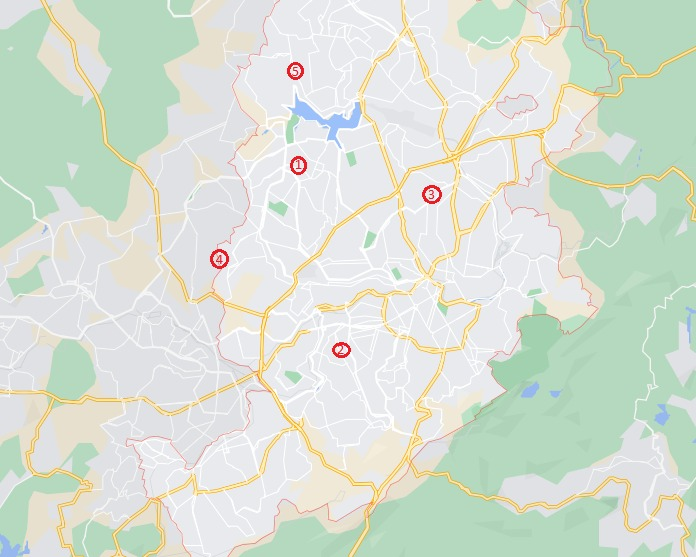
\includegraphics[width=0.5\textwidth]{imagens/grafos1.jpeg}
    \end{figure}
\end{center}

\pagebreak
\subsection{Não Direcionado, Não Ponderado}
A representação do grafo com as arestas ligando cada vértice.
\begin{center}
    \begin{figure}[h!]
        \centering
        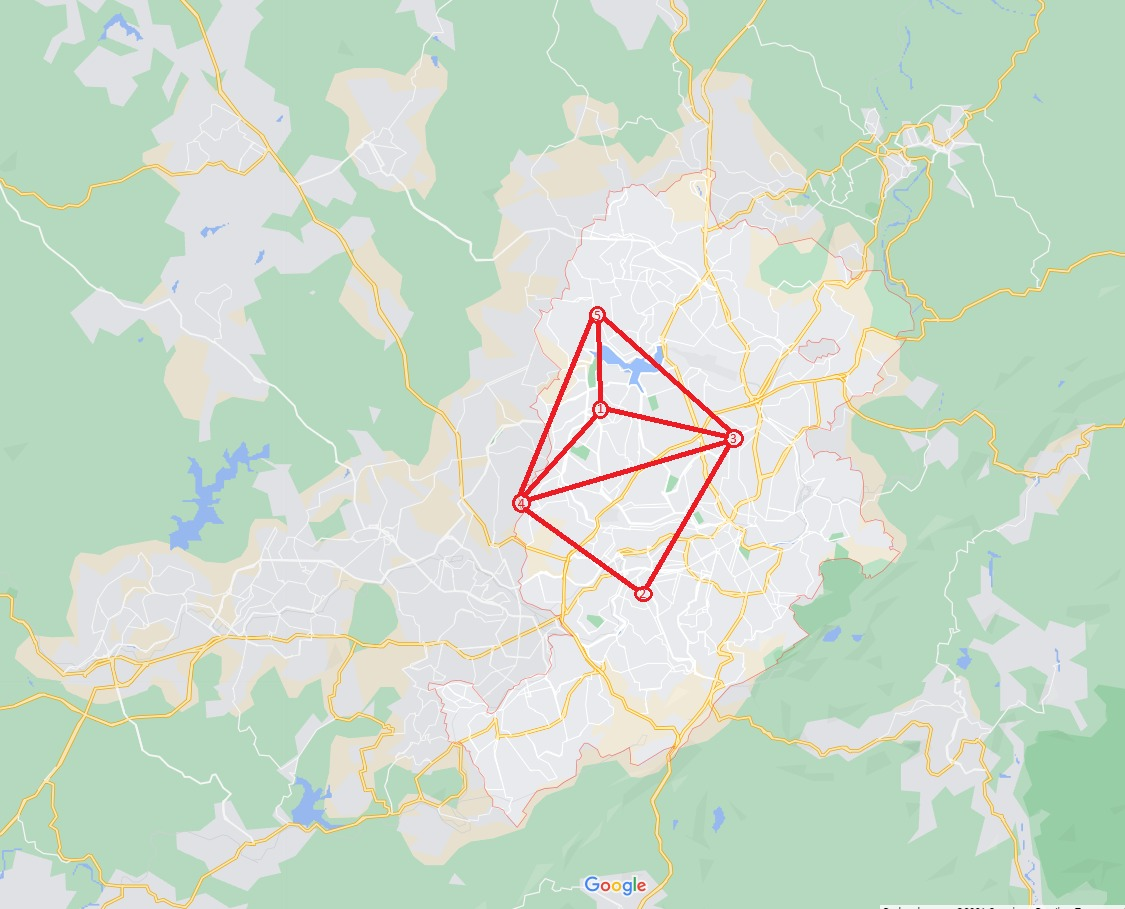
\includegraphics[trim={15cm 10cm 10cm 10cm},clip, width=0.5\textwidth]{imagens/grafos4.jpeg}
    \end{figure}
\end{center}


\subsection{Direcionado, Não Ponderado}
PA representação do grafo com as arestas representando a ligação entre os vértices e, as direções como o fluxo das vias de Belo Horizonte.

\begin{center}
    \begin{figure}[h!]
        \centering
        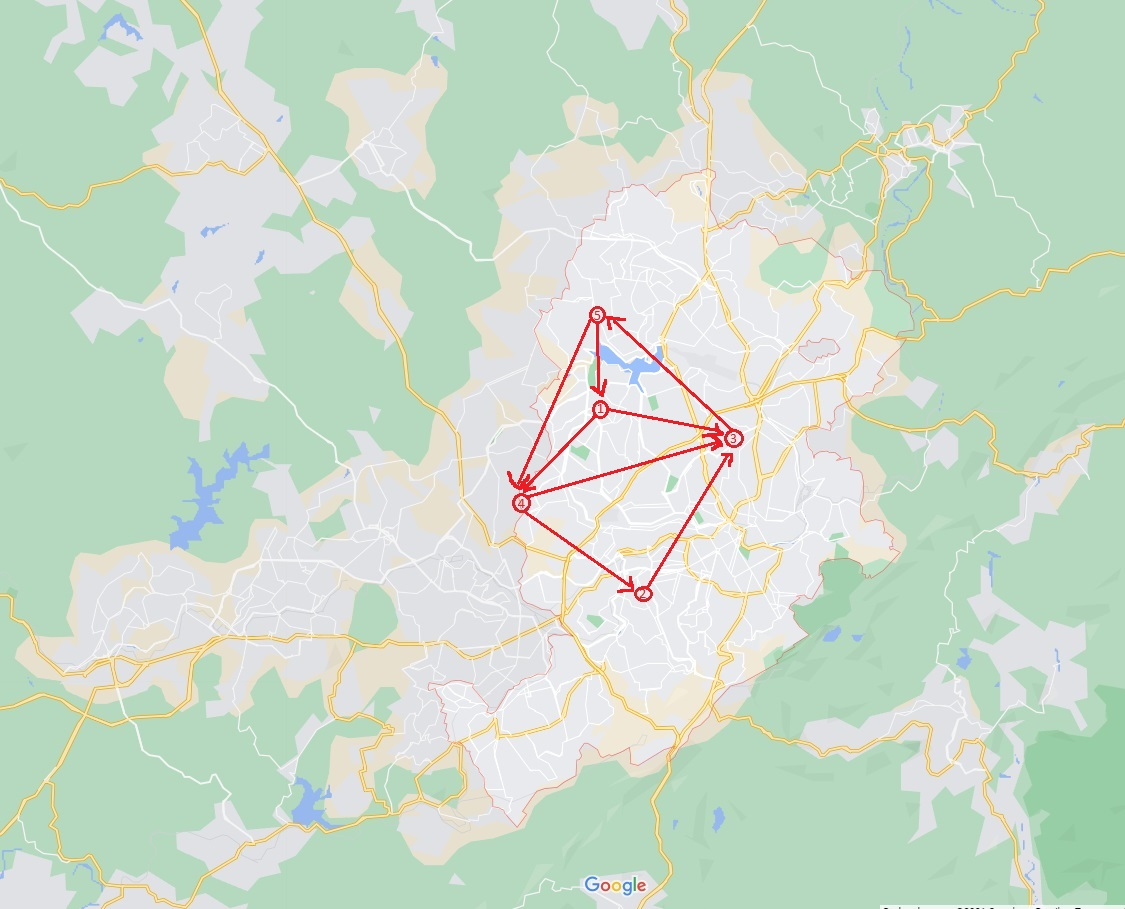
\includegraphics[trim={10cm 7cm 7cm 7cm},clip, width=0.5\textwidth]{imagens/grafos2.jpeg}
    \end{figure}
\end{center}

\pagebreak
\subsection{Não Direcionado, Ponderado}
A representação do grafo com as arestas representando as distâncias entre os vértices desconsiderando o sentido de fluxo das vias de Belo Horizonte.

\begin{center}
    \begin{figure}[h!]
        \centering
        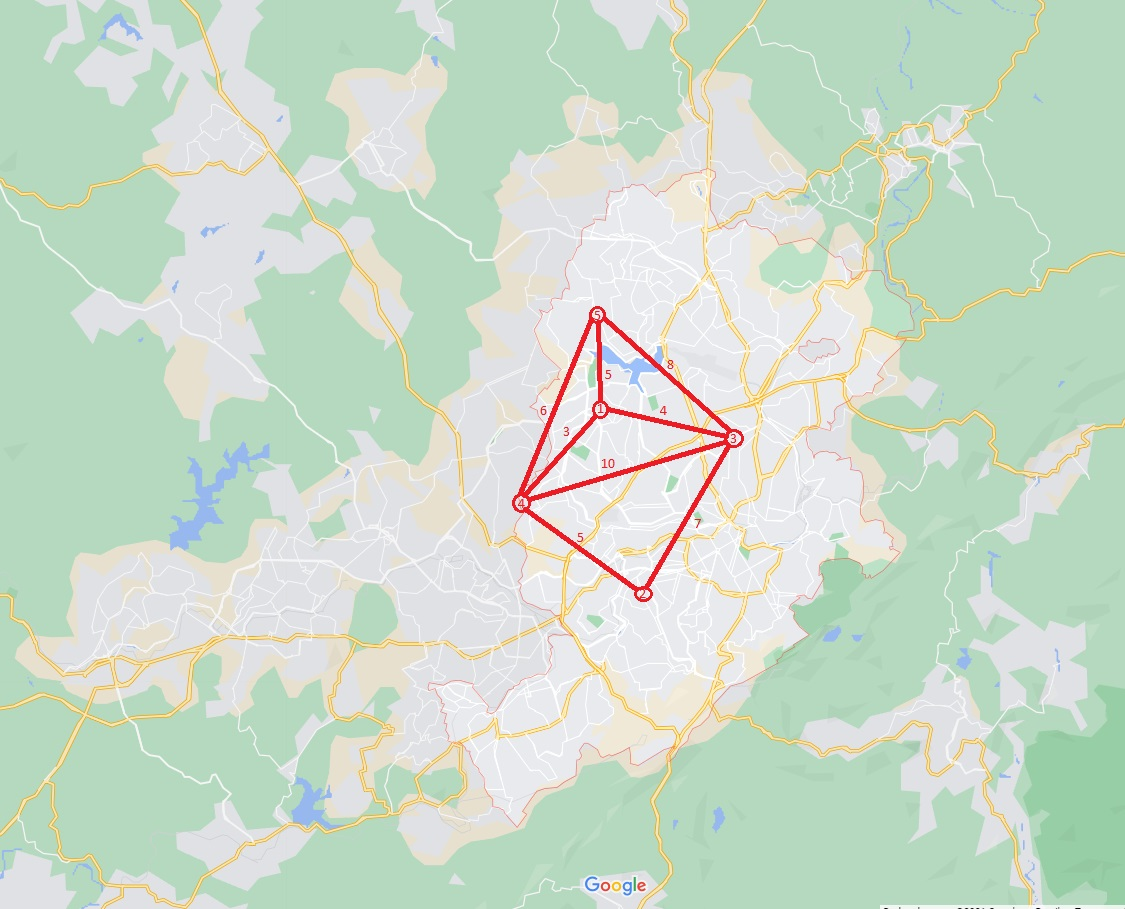
\includegraphics[trim={10cm 7cm 7cm 7cm},clip, width=0.5\textwidth]{imagens/grafos5.jpeg}
    \end{figure}
\end{center}

\subsection{Direcionado, Ponderado}
A representação do grafo com as arestas representando as distâncias entre os vértices considerando o sentido de fluxo das vias de Belo Horizonte.

\begin{center}
    \begin{figure}[h]
        \centering
        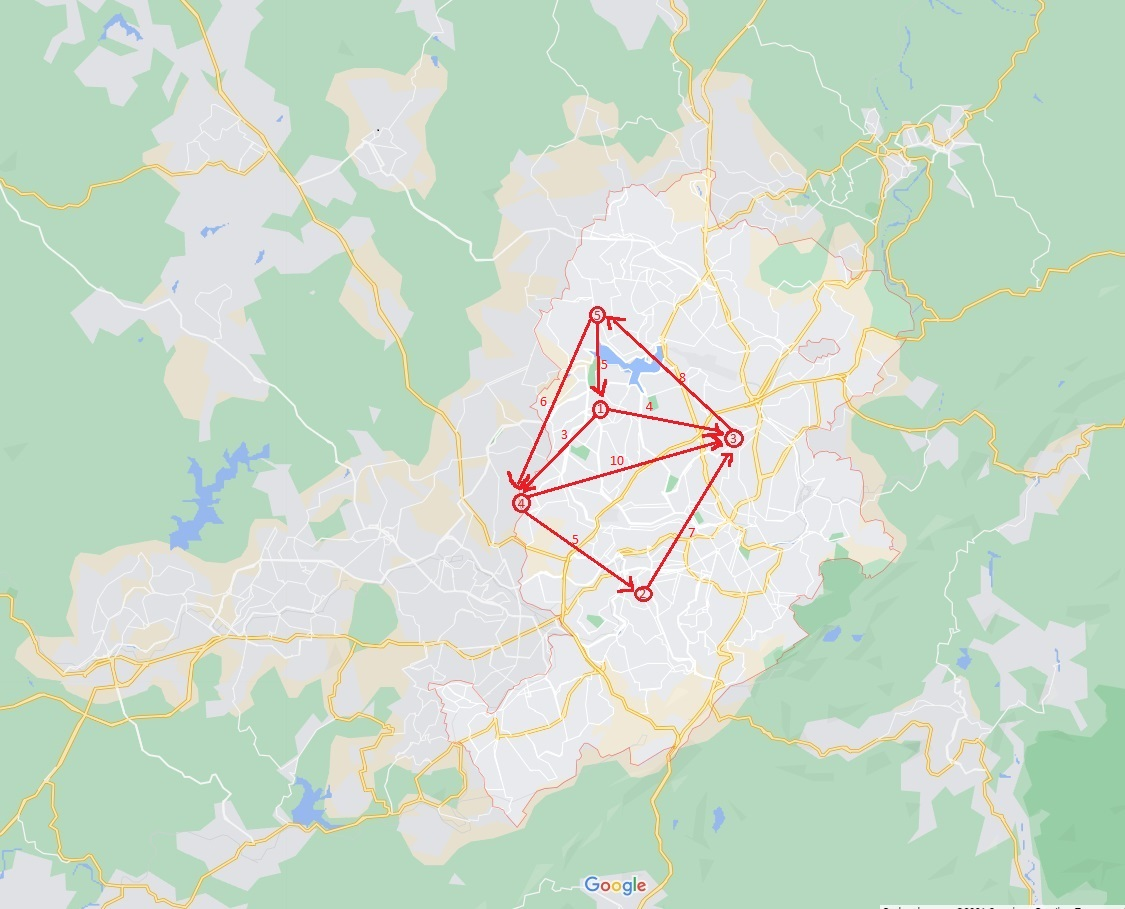
\includegraphics[trim={10cm 7cm 7cm 7cm},clip, width=0.5\textwidth]{imagens/grafos3.jpeg}
    \end{figure}
\end{center}

\section{Implementação}
O Grafo em questão foi implementado no projeto \textit{implementation}, localizado no diretório \textit{lista\_1} em C++ utilizando Cmake como project mananger.

\subsection{Execução}
Para executar o código, precisa-se estar no diretório \textit{lista\_1/build} e digitar o comando \textit{make}, após a compilação, executar o arquivo \textit{./implementation}.

\subsection{Arquivos}
\begin{itemize}
    \item \textbf{\textit{main.cpp:}}
    Arquivo que contem a main e responsável pela criação/execução das listas encadeadas e matrizes.
    \item \textbf{\textit{lista.hpp:}}
    Cabeçalho que contém a classe lista, uma classe genérica que trabalha recebendo células que possuam um ponteiro para a proxima célula.
    \item \textbf{\textit{metodos.hpp:}}
    Cabeçalho que contém métodos diversos para o bom funcionamento dos códigos.
    \item \textbf{\textit{celula.hpp:}}
    Cabeçalho que contém a classe célula base para a utilização da lista
    \item \textbf{\textit{encadeada.hpp:}}
    Cabeçalho que contém a classe genérica CelulaEncadeada que possui uma lista de células e um ponteiro para a proxima encadeada.
\end{itemize}


\end{document}